\section{Ergebnisse}
\label{sec:ergebnisse}
\nocite{lohmoller2013latent}
Zur Evaluierung des Forschungsmodells und der Hypothesen wurde die Partial-Least-Square(PLS)-Methode verwendet. Dabei werden "`die Modellparameter so geschätzt, dass der Anteil der erklärten Varianz der abhängigen Variable und der Indikatoren eines reflektiv gemessenen Konstrukts maximiert wird"' \parencite[S.16]{nitzl2010anwenderorientierte}. Ein besonderer Vorteil der PLS-Methode ist ihre Anwendungsmöglichkeit auch bei verhältnismäßig kleiner Stichprobengröße. Zur Kalkulation einer minimalen Stichprobengröße kommt häufig eine Faustregel zur Anwendung, nach der die Stichprobengröße mindestens das zehnfache des Konstruktes mit der größten Anzahl zu schätzender Parameter sein sollte \parencite[vgl.][S.394]{islam2013investigating}. Dieses Kriterium wird in dieser Studie erfüllt. Zur Analyse wurde die Softwareapplikation SmartPLS \footnote{SmartPLS ist ein Produkt der SmartPLS GmbH und wurde in der Version 3.2.1 genutzt.} verwendet. 

Für die Modellbeurteilung wird zunächst das reflektive Messmodell (äußeres Messmodell) einer Güteprüfung unterzogen. Die Konvergenzvalidität wird anhand der Kriterien Indikatorreliabilität, Konstruktreliabilität und duchschnittlich erfasste Varianz (DEV) kritisch betrachtet, während die Validität mithilfe der Diskriminanzvalidität überprüft wird.

Die Indikatorreliabiltät testet, ob sich ein Indikator für die Messung einer latenten Variable eignet. Eine Faktorladung $\lambda$ > 0,7 gilt als signifikant \parencite[vgl.][S.24]{nitzl2010anwenderorientierte}. Der Wert wird von allen Indikatoren erreicht (siehe Tabelle \ref{tab:Forschungsmodell}). 

Die Konstruktreliabilität $\rho$ untersucht unter Einsatz der internen Konsistenz (Composite reliability (CR)) "`wie gut die Indikatoren eine latente Variable wiedergeben"' \parencite[S.25]{nitzl2010anwenderorientierte}. Ein Wert von $\rho$ $\geq$ 0,6 gilt als akzeptabel \parencite[vgl.][S.212]{ringle2007beurteilung}. Das Messmodell weist $\rho$ > 0,8 auf und liegen damit deutlich über dem Schwellenwert. Nach \textcite[S.320]{chin1998partial} ist dieses Gütekriterium für die interne Konsistenz dem häufig verwendeten Cronbach's Alpha vorzuziehen, da  Cronbach's Alpha bei Verwendung der PLS-Methode zur Unterschätzung der internen Konsistenz neigt.     

Die durchschnittliche erfasste Varianz (DEV) "`setzt den Anteil der erklärten Varianz in Relation zum Messfehler einer latenten Variable"'  \parencite[S.25]{nitzl2010anwenderorientierte}. Ein Wert von DEV $\geq$ 0,5 stellt einen ausreichend hohen Wert dar. Die DEV liegt in dieser Studie mit DEV > 0,7 ebenfalls über dem genannten Schwellenwert und ist somit akzeptabel. Die entsprechenden Werte für die Konstruktreliabilität und die DEV können Tabelle \ref{tab:Übersicht Gütekriterien} entnommen werden. 

Die Diskriminanzvalidilität hingegen "`gibt an, in welchem Ausmaß sich die Indikatoren eines Konstrukts von denen eines anderen Konstrukts unterscheiden"' \parencite[S.26]{nitzl2010anwenderorientierte}. Zur Überprüfung der Diskriminanzvalididtät kann das Fornell-Larcker-Kriterium und die Cross Loadings herangezogen werden.


\begin{table}[h] 
\footnotesize
\caption{Cross Loadings}
\label{tab:Cross-Loadings} 
\begin{tabular}{@{}llllll@{}} \toprule

 & \textbf{Net Benefit} & \textbf{Nutzerzufriedenheit} & \textbf{Servicequalität} & \textbf{Systemqualität} \\ \midrule

Problemorientiertes Denken 	& \textbf{0,930}	& 0,644	& 0,475	& 0,203	\\

Neu erlerntes Wissen	& \textbf{0,763}	& 0,370 	& 0,250 	& 0,237	\\ 

Zufriedenheit 			& 0,688 		& \textbf{0,907} & 0,541	& 0,339	\\

Nutzereinstellung		& 0,293		& \textbf{0,763}	 & 0,526 & 0,168 \\
 
Verfügbare Beratung		& 0,479 		& 0,546 	&\textbf{0,913}	& 0,257		\\

Onlinehilfe 			& 0,317 		& 0,529	& \textbf{0,794}	& 0,493 		\\

Tutorenunterstützung	& 0,369 		& 0,562 	& \textbf{0,887}	& 0,168		\\ 

Einfache Bedienung		& 0,155 		& 0,227 	& 0,220	& \textbf{0,856}	\\ 

Gute Funktionalitäten 	& 0,258 		& 0,224	& 0,325	& \textbf{0,876} 		\\ 
 
Persönliche Informationen & 0,216 	& 0,334 	& 0,322	& \textbf{0,828}	\\	
		 
 \bottomrule
 
\end{tabular}	
\end{table}



Bei ersterem wird die Wurzel der DEV einer latenten Variable verglichen mit jeder Korrelation dieser latenten Variable mit einer anderen latenten Variablen und sollte stets größer sein \parencite[vgl.][S.26]{nitzl2010anwenderorientierte}. Das Fornell-Larcker-Kriterium wird in dieser Studie erfüllt (siehe Tabelle \ref{tab:Fornell-Larcker-Kriterium}). Die Cross Loadings können Tabelle \ref{tab:Cross-Loadings} entnommen werden. Ein Indikator sollte dabei die stärkste Beziehung mit dem ihm zugeordneten Konstrukt aufweisen \parencite[vgl.][S.26]{nitzl2010anwenderorientierte}, was ebenfalls erfüllt ist.   \nocite{fornell1981evaluating}

\begin{figure}[h]
\centering
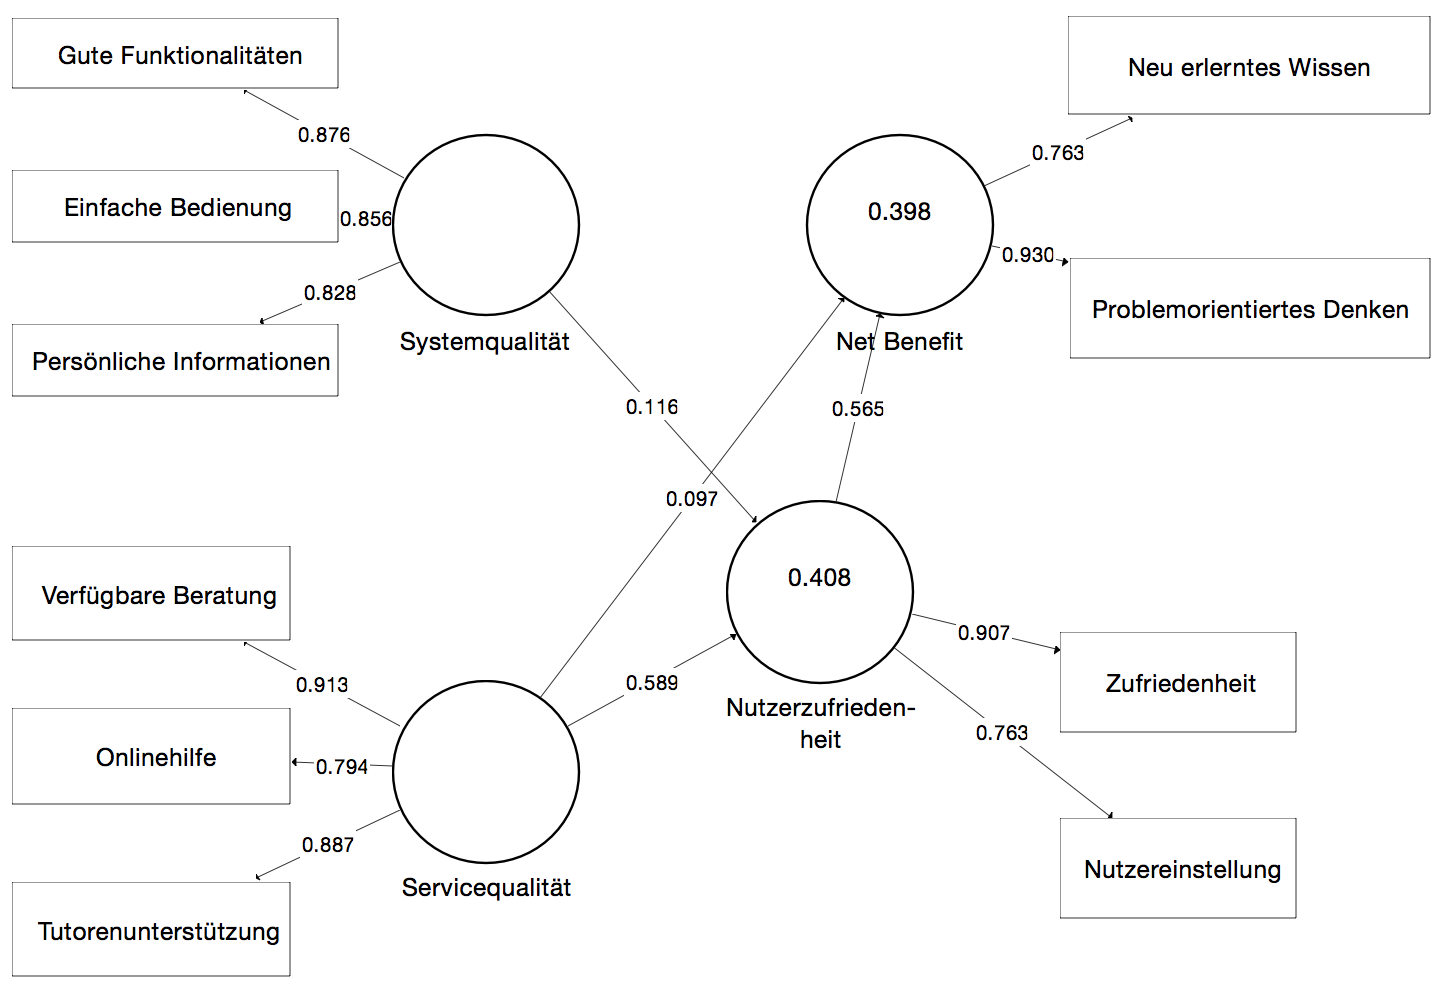
\includegraphics[width=1\textwidth]{Grafiken/pls_bw_3.png}
\caption{PLS Modellergebnisse}
\label{PLS Modellergebnisse}
\end{figure}


Das Messmodell erfüllt damit alle Gütekriterien. Zur Beurteilung des Strukturmodells (inneres Messmodell) werden das Bestimmtheitsmaß R$^2$, die Pfadkoeeffizienten, die Effektstärke f$^2$ und die Prognoserelevanz Q$^2$ herangezogen.  

Die Werte für das Bestimmtheitsmaß R$^2$ sind in Tabelle \ref{tab:Übersicht Gütekriterien} enthalten. Das Bestimmtheitsmaß "`gibt den Anteil der erklärten Varianz im Verhältnis zur Gesamtvarianz an."' \parencite[S.32]{nitzl2010anwenderorientierte} Eine Einteilung relevanterer Schwellenwerte wurde von \textcite[S.323]{chin1998partial} in einer Studie ermittelt. Die Werte für R$^2$ von 0,67, 0,33 und 0,19 wurden in "`substanziell"', "`mittelgut"' und "`schwach"' eingeteilt. In dieser Studie sind die R$^2$ dementsprechend als "`mittelgut"' (Nutzerzufriedenheit: 0,387 / Net Benefit: 0,369) einzustufen.

Als Schwellenwerte für die Effektstärke f$^2$ wurden von \textcite[S.316f.]{chin1998partial} 0,02, 0,15 bzw. 0,35 ermittelt. Diese sagen aus, ob eine unabhängige latente Variable einen geringen, mittleren bzw. großen Einfluss auf eine abhängige latente Variable hat. Demnach weist Nutzerzufriedenheit auf den Net Benefit (f$^2$=0,320) einen mittleren Einfluss und Serviceualität auf Nutzerzufriedenheit (f$^2$=0,517) einen großen Einfluss aus. 

Die Pfadkoeeffizienten $\gamma$ geben die Stärke der Kausalbeziehung zwischen den latenten Variablen an. Sie können Werte zwischen -1 und 1 annehmen. Ein Wert Nahe 0 gilt als schwach. Als signifikant wird ein Wert kleiner -0,2 oder größer 0,2 angesehen \parencite[vgl.][S.11]{chin1998commentary}. In dieser Studie haben dementsprechend die Nutzerzufriedenheit auf den Net Benefit ($\gamma$ = 0,565; p < 0,001) und die Servicequalität auf die Nutzerzufriedenheit ($\gamma$ = 0,589; p < 0,001) einen signifikant Einfluss (siehe Abbildung \ref{PLS Modellergebnisse}). Die mithilfe der Bootstrapping-Methode von SmartPLS ermittelten T-Werte bestätigen die Signifikanz der beiden Pfadkoeffizienten. Systemqualität auf Nutzerzufriedenheit ($\gamma$ = 0,116) und Servicequalität auf Net Benefit ($\gamma$ = 0,097) haben hingegen keinen signifikanten Einfluss. 

\nocite{geisser1974predictive}

Das Geisser-Stone-Kriterium stützt sich auf eine von Geisser und Stone entwickelte Methode zur Wiederverwertung von Daten und sieht eine ausreichende Prognoserelevanz als gegeben, wenn Q$^2$ > 0 \parencite[vgl.][S.35]{nitzl2010anwenderorientierte}. Die Berechnung erfolgte mithilfe der Blindfolding-Methode in SmartPLS. Das Kriterium wird in dieser Studie erfüllt (siehe Tabelle \ref{tab:Übersicht Gütekriterien}).
 

\begin{table}[h] 
\footnotesize
\caption{Übersicht Gütekriterien}
\label{tab:Übersicht Gütekriterien} 
\begin{tabular}{@{}llllll@{}} \toprule

\textbf{Faktor} & \textbf{DVE} & \textbf{CR} & \textbf{R$^2$} & \textbf{Q$^2$} \\ \midrule

 Net Benefit 		& 0,724 		& 0,838 		& 0,378 		& 0,239 		 \\
 
 Servicequalität 	& 0,750 		& 0,900 		& 			& 			 \\

 Systemqualität 	& 0,729 		& 0,890 		& 			& 			 \\

 Nutzerzufriedenheit & 0,703 	& 0,824 		& 0,389 		& 0,254		 \\ \bottomrule
\end{tabular}	
\end{table}



\begin{table}[h] 
\footnotesize
\caption{Fornell-Larcker-Kriterium}
\label{tab:Fornell-Larcker-Kriterium} 
\begin{tabular}{@{}llllll@{}} \toprule

 & \textbf{Net Benefit} & \textbf{Nutzerzufriedenheit} & \textbf{Servicequalität} & \textbf{Systemqualität} \\ \midrule

 Net Benefit 			& \textbf{0,851}		& 			& 		&  		\\
 
 Nutzerzufriedenheit 	& 0,626 		& \textbf{0,838}		& 		& 			\\

 Servicequalität 		& 0,452 		& 0,629 		& \textbf{0,866}	& 		 \\

 Systemqualität 		& 0,248 		& 0,319 		& 0,345 	& \textbf{0,854} \\ 
 
 \bottomrule
\end{tabular}	
\end{table}












